% !TEX root = ../main.tex

\chapter{绪论}\label{chap:introduction}

\section{研究背景和意义}

医疗图像分割技术是计算机视觉和模式识别技术应用在诸如X-Ray CT(X光计算机断层扫描成像)、MRI(磁共振成像)和Ultrasound(超声成像)等医疗图像上,
针对特定的目标,譬如肺部动脉/静脉血管、乳腺肿块,肺癌结节,进行逐体素(Voxel)的分类。本文聚焦肺部CT扫描图像,研究肺部支气管树状结构的气道分割提取技术。


肺部和呼吸系统疾病对人体健康威胁巨大,自2019年底、2020年初爆发的全球性新冠肺炎COVID-19疫情严重冲击人类的公共卫生与生命健康。三年多来,世界各国在抗击新冠肺炎疫情方面付出了惨重的生命代价和社会经济损失。新型冠状病毒经由空气为媒介传播,通过呼吸道进入肺部并感染细胞。包括肺癌在内的一些肺部疾病,慢性
阻塞性肺疾病(COPD)\cite{fetita2004pulmonary}、急性呼吸窘迫综合症\cite{howling1998significance}、闭塞性细支气管炎\cite{shaw2002role}、特发性肺纤维化\cite{wu2019computed}、肺挫伤\cite{li2019application}等导致肺支气管气道树的形态学变化。
支气管气道树的形态学三维模型通过从基于CT扫描的肺部图像中精确分割出来,是分析包括哮喘、支气管扩张和肺气肿在内的肺部疾病的关键步骤。测量精确分割出来的支气管的气道管腔
尺寸和管壁厚度,可以用于辅助诊断肺栓塞\cite{estepar2013computed}, 揭示慢性阻塞性肺部疾病COPD患者的异常病症。除了上述这些疾病诊断治疗之外,本文研究肺部支气管气道
树分割的一个直接动因是为了开发支气管镜和支气管导航与活体检测的手术机器人。手术机器人驱动细长柔性的支气管镜器械,伸入支气管,沿着气道导航至疑似(肺部)病灶部位,对
病灶处细胞进行活体采样返回,进而化验诊断出疾病。本文作者所在的工作单位就在开发国产的支气管镜导航/检测的手术机器人,而支气管气道树的精确分割就是非常重要的前置研发步骤。
构建出支气管气道树的分割模型后,输入患者的肺部CT扫描图像数据,就可以输出包含精确的三维空间信息的支气管气道树结构。将这个支气管气道树的结构模型“喂给”支气管镜导航机器人
(Bronchoscopy and endobronchical navigation robot),在医生的监视与操纵下,机器人就可以被引导进入支气管管腔内,进行疾病的诊断与治疗了。

{\heiti 支气管气道树的分支结构。} 本文研究支气管气道树的分割,有必要先了解一下支气管数状结构的气道解剖结构。从图\ref{fig:branches_of_bronchial_tree}中可以看出,支气管气道树的分支结构非常复杂,从气管(Trachea)往下分为左、右两支主支气管(Main bronchus),左右两支主支气管各自分岔为上叶支气管(Superior lobar bronchus)、中叶支气管(Middle lobar bronchus)和下叶支气管(Inferior
 lobar bronchus)。在每个肺叶内,起于肺叶的支气管继续分岔为多个肺段支气管(Segmental bronchi)。肺段支气管最后分为更细小的支气管到达肺泡。

\begin{figure}[!htp]
	\centering
	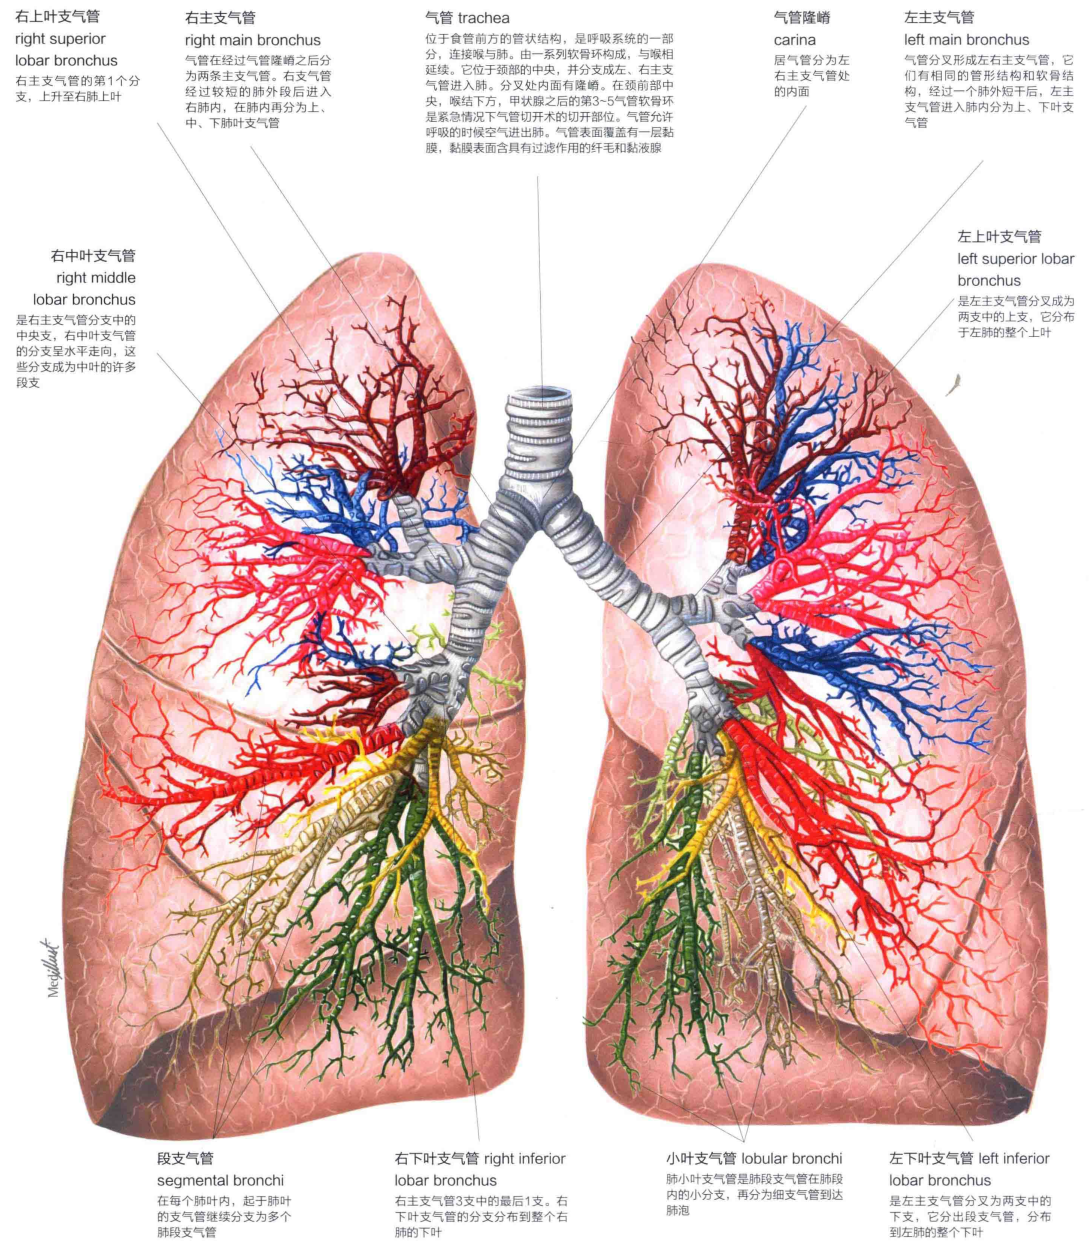
\includegraphics[width=0.9 \textwidth]{branches_of_the_bronchial_tree}
	\bicaption[肺部支气管气道树的分支结构]
		{肺部支气管气道树的分支结构\parencite{humananatomy2nd}}
		{The branch structure of pulmonary bronchial airway tree}
	\label{fig:branches_of_bronchial_tree}	
\end{figure}

如此繁复,从粗到细不断分化,面对如此稠密细小的支气管气道树,进行分割前需要经验丰富的临床专家进行非常细粒度的标注。手工标注耗费大量时间,
成本高昂且支气管越细小,标注越困难,易于出错。 标注任务艰巨繁重,急需开发新的算法或模型来帮助临床医生解决支气管气道树分割的问题。

\section{本研究的应用前景}\label{sec:application_prospect}

肺部支气管气道树的自动化分割是呼吸系统肺部疾病诊断治疗的一个重要问题和研究领域,在实际应用中具有非常重要的作用,提高医疗技术水平。当前,在
作者所在的医疗机器人行业,本研究项目有如下的应用前景:
\begin{itemize}
	\item {\heiti 导管手术机器人 }
	由于肺部支气管气道树三维模型具有精确的空间位置信息,CT扫描建立的坐标系赋予DICOM医疗图像每个像素都有相应的坐标位置信息,如图\ref{fig:coordinate}所示。
	\begin{figure}[!htp]
		\centering
		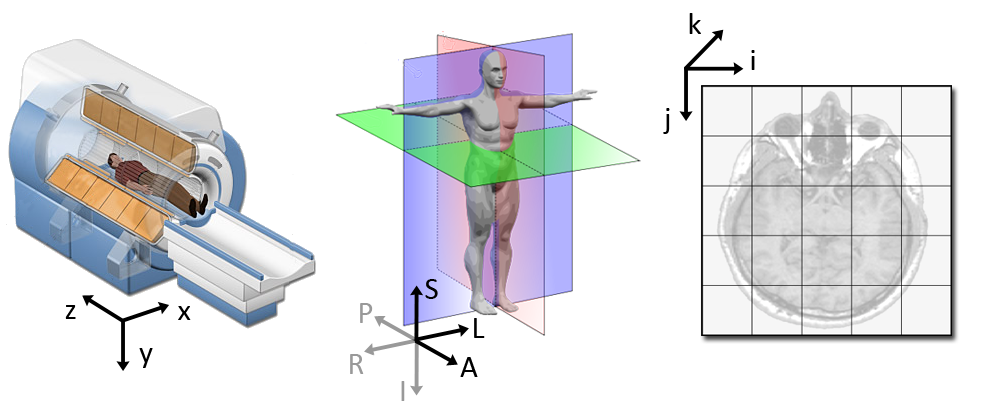
\includegraphics{Coordinate_sytems.png}
		\bicaption[CT扫描仪坐标系,人体坐标系和DICOM图像坐标系对应关系]
			{CT扫描仪坐标系,人体坐标系和DICOM图像坐标系对应关系\parencite{ctcoordinatesys2022, adaloglou2020dicomcoordinates}}
			{CT scanner, human body and DICOM imaging coordinates}
		\label{fig:coordinate}
	\end{figure}
	这样,分割出来的支气管气道树三维模型其每一个体素(Voxel)就具有精确的坐标位置信息,就可以计算出支气管管腔的中心线位置。
	
	导管机器人就是沿着管腔中心线的路径移动,导航至靶标位置。目前,美国Intuitive Surgical Company已经开发出肺部导管机器人ION,并投入了临床应用。
	\begin{figure}[!htp]
		\centering
		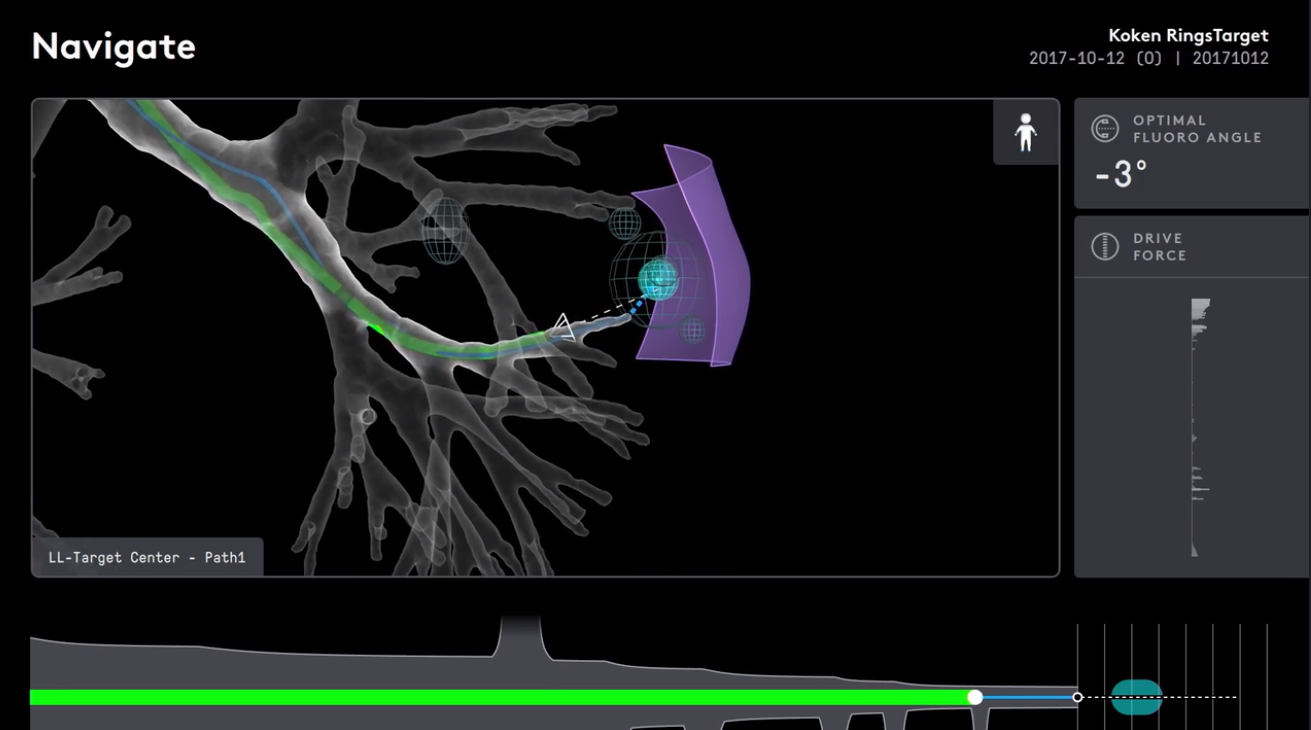
\includegraphics[width=0.45 \textwidth]{ION_robot_navigating}
		\hspace{2mm}
		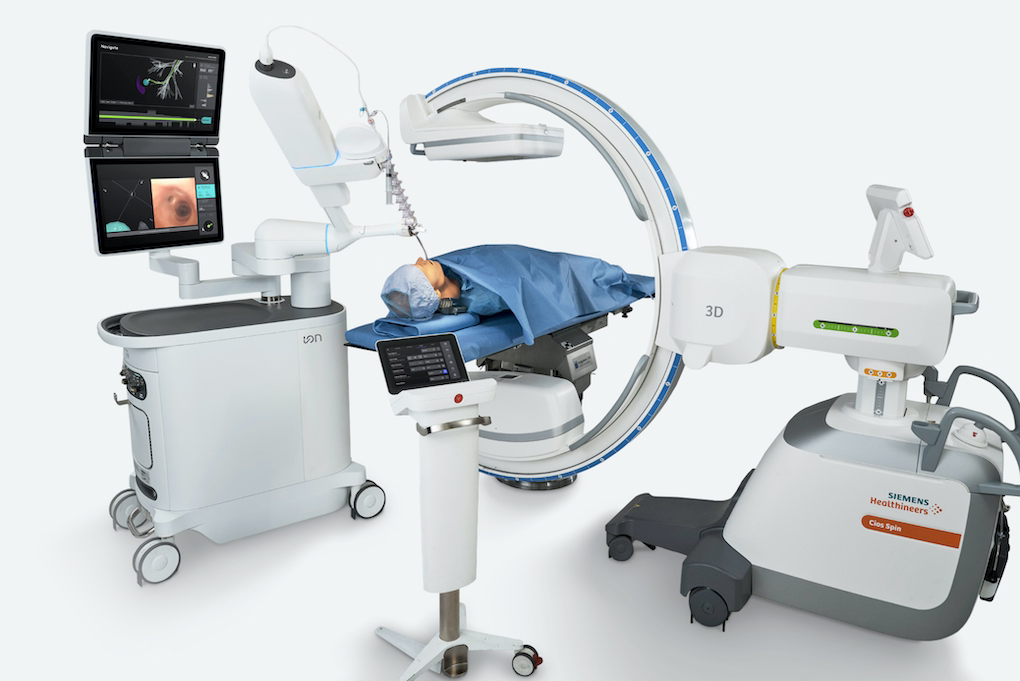
\includegraphics[width=0.45 \textwidth]{ION_bronchoscopy_robot.jpg}
		\bicaption[ION肺部导管机器人]
			{ION肺部导管机器人\parencite{ionrobot2021}}
			{ION bronchoscopy robot}
		\label{fig:ION_robot}
	\end{figure}
	
	作者所在的工作单位正在开发国产的肺部导管机器人,已经完成全国首例机器人辅助经支气管镜肺结节活检手术。
	
	当然导管手术机器人除了依赖支气管气道树三维模型导航,还需要辅助术中实时定位、支气管镜视觉导航的技术。
	
	
	\item {\heiti 智慧医疗辅助诊断}
	基于CT扫描图像的医疗图像分割需要高质量的标注数据,这很大程度上依赖经验丰富的临床医生/专家的专业知识。 为了减轻临床医生的标注压力和负担,同时亦为了减少误诊和漏诊
	的情况发生,医疗图像分割技术在医学辅助诊断上已经获得越来越多的应用。 具体到支气管气道树分割技术上,已经被用来辅助诊断一些慢性阻塞性肺部疾病COPD, 支气管扩张和肺气肿
	等一些肺部疾病。 随着AI图像分割技术的不断的进步,可以辅助临床医生更准确更高效地诊断疾病,逐渐达成智慧医疗,提高医疗技术水平和能力。
\end{itemize}



\section{研究现状和发展趋势}


图像分割技术已经发展很多年,从过去十年的发展来看,图像分割技术的发展经历了传统的图像分割方法和基于深度学习的分割方法2个阶段。传统的图像分割方法产生了一些比较经典的算法,
诸如基于阈值的最大类间方差Otsu方法\cite{otsu1979threshold},基于聚类的K-Means算法\cite{macqueen1965some}等。而随着近年来深度学习的发展,深度学习应用于图像分割
则是涌现了大量优秀的分割方法。Jonathan Long等人\cite{long2015fully}首次提出的全卷积网络(Fully Convolution Neural Network, FCN), 最经典的当属Olaf Ronneberger等人\cite{ronneberger2015u}提出的UNet结构,以及在UNet基础上改进提出的V-Net\cite{milletari2016v}结构模型、U-Net++\cite{zhou2019unet++}
结构模型,还有针对医疗影像这类三维体数据的分割模型3D UNet结构\cite{cciccek20163d},诸如这些基于深度学习的图像分割模型,其性能、精度、鲁棒性等指标都在不断进步,发展非常活跃。

下面分别介绍传统的图像分割方法、基于深度学习的图像分割方法和具体针对肺部支气管气道树的分割方法,了解他们的基本思想和发展趋势。

	\subsection{传统的图像分割方法}
	
	传统图像分割的方法是根据图像特征设计相应的算法对每个像素点进行分类,这些图像的特征包括颜色、纹理、亮度和形状等,其本质是根据特定标准确定一个合理的阈值,将每一个
	像素点与此阈值比较,以确定每一个像素点的分类。综合分析传统的图像分割方法,我们可以总结出如下的划分:
	\begin{enumerate}
		\item 阈值法
		
		阈值法是根据图像的灰度特征信息进行与阈值比较的计算。对欲分割的图像设定一个或多个(不同)的阈值,然后将图像上的每一个像素点与阈值进行比较,得到每个像素点所属的
		类别。这方面主要的工作有Sauvola法\cite{sauvola2000adaptive}、最大类间方差Otsu法\cite{otsu1979threshold}等。医疗图像(DICOM格式\cite{mustra2008overview})都是典型的灰度图\ref{fig:medical_image}。
		\begin{figure}[!htp]
			\centering
			\begin{subfigure}{\textwidth}
				\centering
				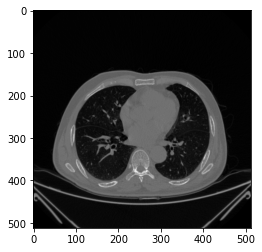
\includegraphics[scale=0.5]{DICOM image(axial view)}
				\caption{轴向面视图}
			\end{subfigure}
			
			\vspace{2mm}
			
			\begin{subfigure}{\textwidth}
				\centering
				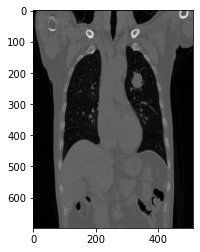
\includegraphics[scale=0.5]{DICOM image(coronal view)}
				\caption{冠状面视图}
			\end{subfigure}
			\bicaption[医疗图像(DICOM格式的灰度图)]
				{医疗图像(DICOM格式的灰度图)}
				{Medical image in DICOM format}
			\label{fig:medical_image}
		\end{figure}
		
		\item 区域法
		
		区域法是根据像素的灰度和纹理信息,以区域一致性规则进行分割。其包括:区域生长法、区域分裂、区域合并法。区域生长法通过指定一个种子点,向生长区域不断地添加满足
		约束条件的新的像素,直到填满或无法再添加。这些新添加进来的像素即属于一个类别,在不同的生长区域的像素从属于不同的类别。区域法初始形式简单,计算速度也快,它比较
		适合灰度均匀的图像分割。
		
		\item 聚类法
		
		聚类方法则根据像素间的特征相似程度进行迭代式的分类,将特征值相近的一组像素归为一个类别,然后计算这一组像素的中心位置。通过不断更新迭代直到完成所有像素的分类。
		这种方法的代表性工作便是K-Means算法\cite{macqueen1965some},聚类法使同类像素样本尽可能相近,而异类像素样本则拉大差异。聚类法的实现较为简单,但缺点就是
		对噪声很敏感,稍微不同的聚类中心和类别选择等因素都会导致分割结果差异,鲁棒性较差。
		
		\item 图论法
		
		图论法源于聚类的分割方法,它是将图像转换成带权重的无向图,将无向图划分为各种子图,使每个子图内部保持最大相似性,而子图之间则是差异尽可能大,每个子图代表
		一个类别。相关的图论分割方法就有归一化图分割、最小图分割、迭代式图分割等。
	\end{enumerate}
	
	\subsection{基于深度学习的图像分割方法}
	
	传统的图像分割方法围绕着图像的某一个具体特征进行精心挑选,设计与之匹配的算法,不具备广泛性和普遍性。 对于医疗的CT扫描图像,如前文图\ref{fig:medical_image}
	所述的都是对比度小的灰度图,传统的图像分割方法对于医疗图像不再适合。
	
	近年来随着深度学习技术在计算机视觉领域的应用,飞速发展并取得显著的进步。 基于深度卷积神经网络的语义分割方法对图像中的所有像素进行精确预测,预测像素属于哪一个类别
	的概率,赋予其标签,通过不断地迭代,从而分割出来图像。自美国加州大学UC Berkeley的Jonathan Long等人\cite{long2015fully}首次提出端到端、像素到像素的全卷积网络
	Fully Convolution Networks for Semantic Segmentation,取得的图像分割效果明显超过以往传统的图像分割法。以此为标志,打开了深度学习在图像分割领域应用的新通
	道。全卷积网络FCN由多个卷积层和池化层组合而成,学习图像中每个像素的语义信息,最后生成像素级的类别概率预测图。
	\begin{figure}[!htp]
		\centering
		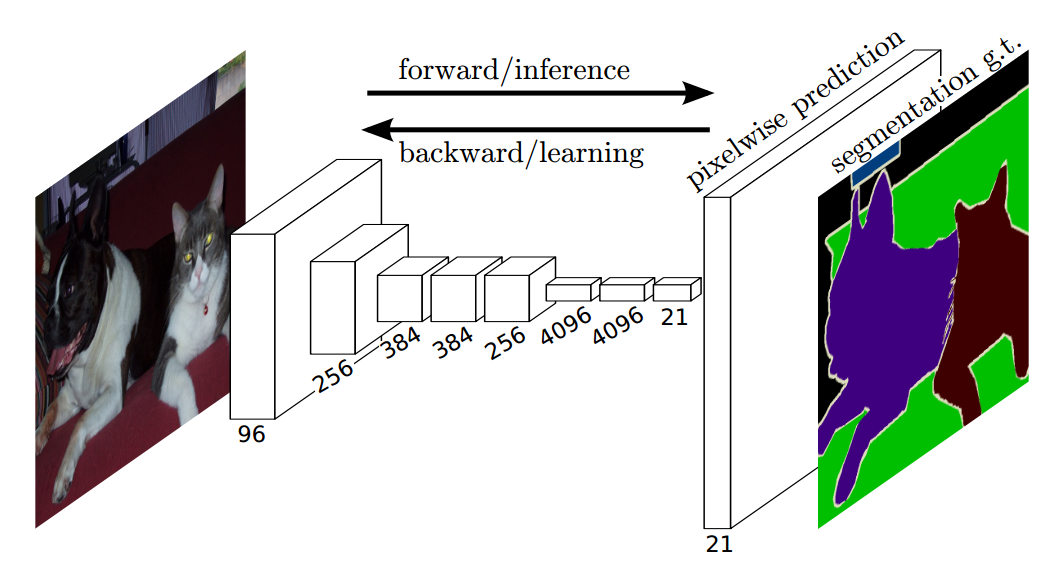
\includegraphics[width = 0.5 \textwidth]{FCN网络的结构}
		\bicaption[FCN网络的结构]
			{FCN网络的结构\cite{long2015fully}}
			{The structure of Fully Convolution Networks}
		\label{fig:FCN}
	\end{figure}
	
	但由于下采样路径上图像分辨率显著被降低,使得最后的预测结果比较粗糙。正如图\ref{fig:FCN}中分割结果只能看到2个物体的轮廓,无法看出是一只猫或是一只狗。在此基础上,
	Hyeonwoo Noh等人\cite{Noh2015LearningDN}添加进去了上采样路径,亦即反卷积Deconvolution,同步加入反池化Unpooling,将图像分辨率逐步恢复到原来的分辨率。
	\begin{figure}[!htp]
		\centering
		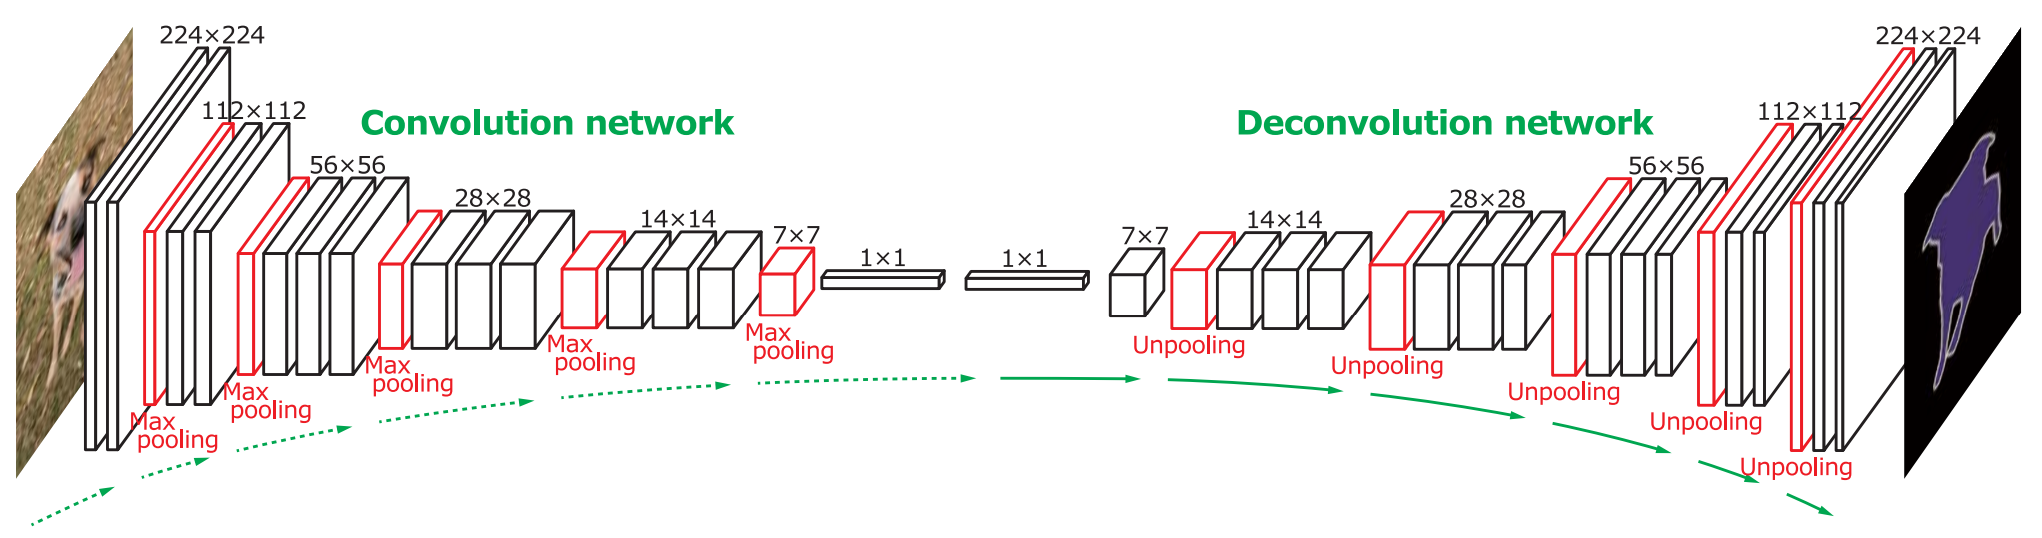
\includegraphics[width = 0.7 \textwidth]{Convolution_and_Deconvolution_network}
		\bicaption[卷积下采样路径 vs. 反卷积上采样路径]
			{卷积下采样路径 vs. 反卷积上采样路径\cite{Noh2015LearningDN}}
			{Convolutuion in down-samping path vs. Deconvolution in up-samping path}
		\label{fig:conv_deconv}
	\end{figure}
	\begin{figure}[!htp]
		\centering
		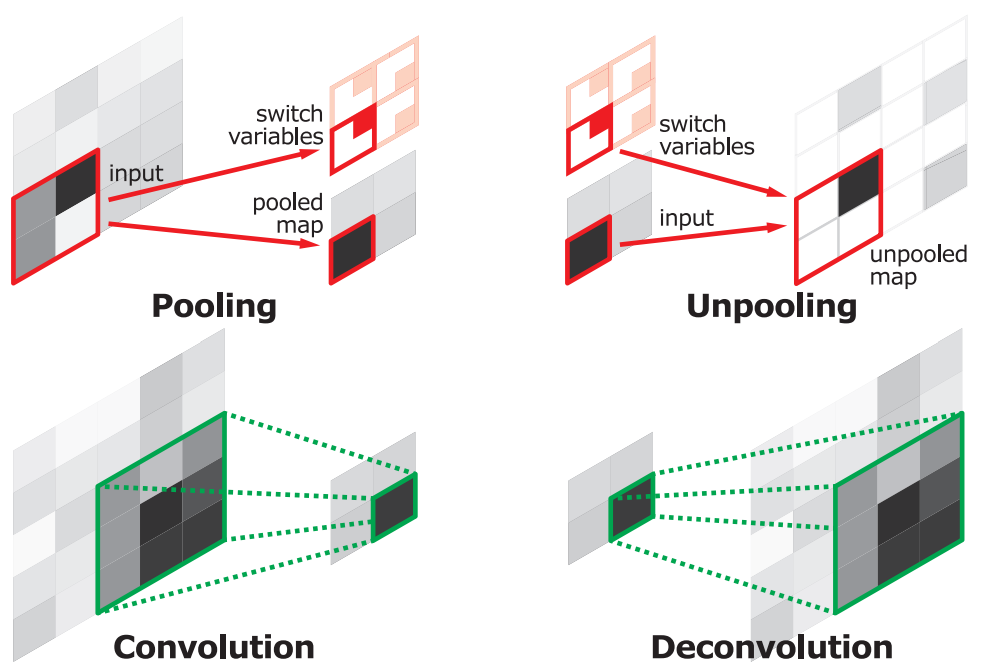
\includegraphics[width=0.6 \textwidth]{Deconvolution_and_unpooling_operations}
		\bicaption[卷积与反卷积,池化与反池化的操作]
			{卷积与翻卷积、池化与反池化的操作\cite{Noh2015LearningDN}}
			{The operations of convolution/deconvolution, and pooling/unpooling}
		\label{fig:conv_deconv_pooling_unpooling}
	\end{figure}
	
	图\ref{fig:conv_deconv}中的Convolution network与Deconvolution network也分别被成为编码器Encoder与解码器Decoder,这两条对称路径构成了Encoder-Deconder
	图像语义分割网络架构。
	
	后来,Olaf Ronneberger等人\cite{ronneberger2015u}则进一步改进,保留下采样路径用于提取深度特征信息,而在上采样路径则加入了跳跃连接,将下采样获取的深度特征信息
	跳跃过来与上采样拼接起来,实现特征图融合。这就是经典的U-Net网络结构。U-Net网络实现了更精细的图像语义分割结果。
	
	\begin{figure}[!htp]
		\centering
		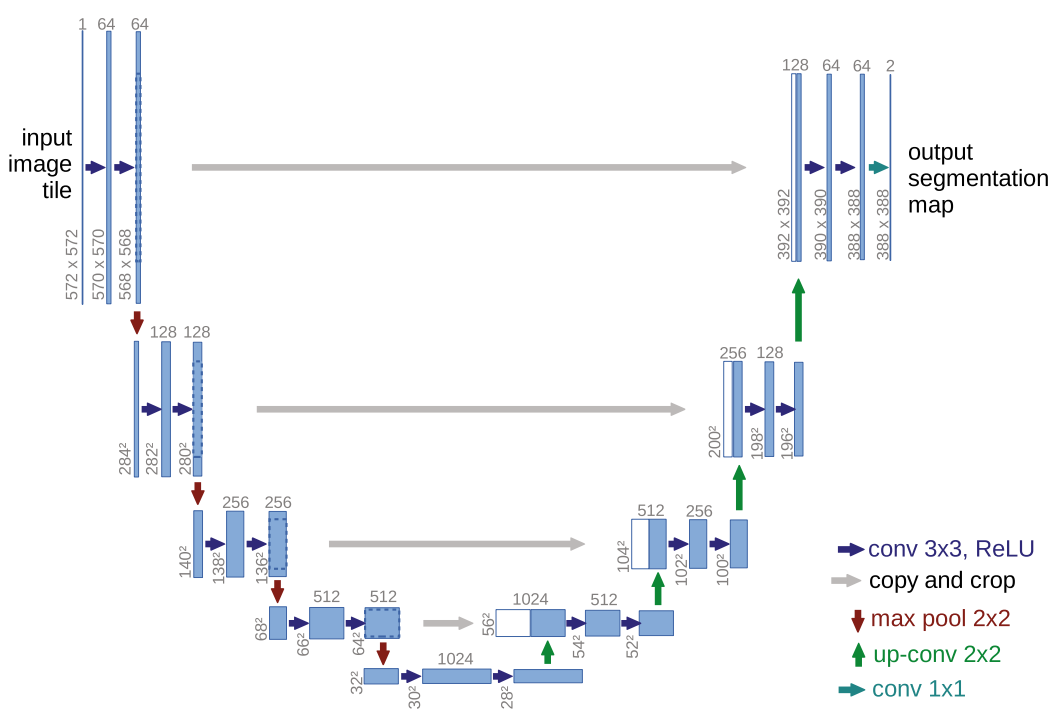
\includegraphics[width=0.7\textwidth]{UNet_architecture}
		\bicaption[经典的图像分割U-Net网络结构]
			{经典的图像分割U-Net网络结构\cite{ronneberger2015u}}
			{The classic U-Net architecture for image segmentation}
		\label{fig:UNet}
	\end{figure}
	
	U-Net网络目前已成为医疗图像分割任务的基础网络,有很多研究人员在U-Net基础上改进,应用在医疗图像的分割。比如肝脏、肺癌结节、乳腺肿块等不同的疾病。Li Xiaomeng等人
	\cite{Li2017HDenseUNetHD}提出一种基于U-Net混合式的稠密连接的新型网络结构H-DenseUNet用于肝癌的医疗CT图像的分割。它将UNet的保留低卷积层的细节特征,UNet网络
	越来越深的层次增加了训练的长耗时,而H-DenseUNet又可以解决这些深层网络的长耗时训练困难。
	
	医疗CT扫描图像基本上都是三维体数据,基于此又引申发展出3D CNN, Jose Dolz等人\cite{Dolze3DFCN}就提出了3D Fully convolutional networks, {\"O}zg{\"u}n {\c{C}}i{\c{c}}ek等人\cite{cciccek20163d}则提出3D UNet用于稠密的体数据分割。如此众多的分割网络,各个作者在UNet的基础上加上自己的创新,形成一个个独具特色的新型
	网络结构。那有没有一种广泛通用的网络来做图像分割呢? Mathias Perslev等人\cite{PerslevGeneralUNetFusion}就提出了这样的一个想法和实施方案
	One Network to segment them all一种通用	的轻量级的网络结构来精确分割3D图像。它是在UNet网络之后再加上一个Fusion model实现的。
	\begin{figure}[!htp]
		\centering
		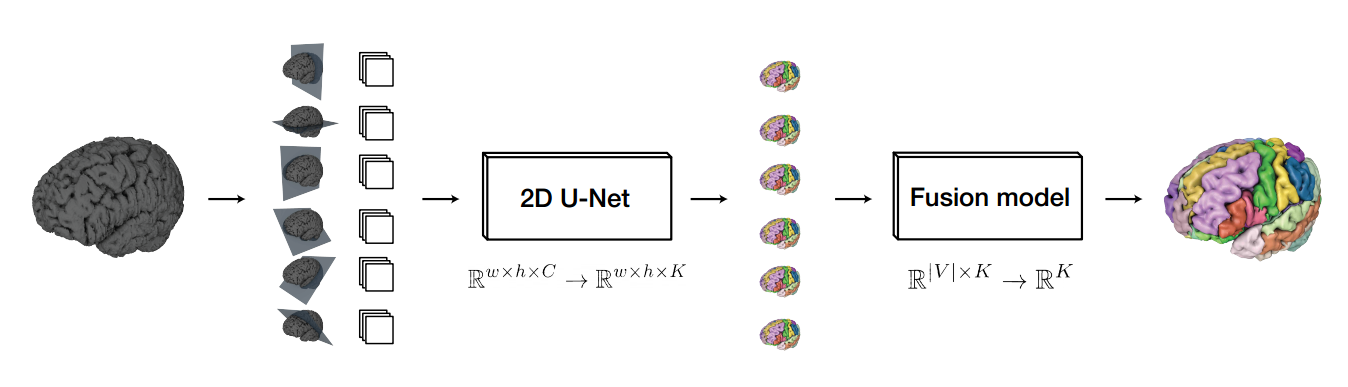
\includegraphics[width=0.8\textwidth]{Genral_UNet}
		\bicaption[一种通用的轻量化的UNet网络]
			{一种通用的轻量化的UNet网络\cite{PerslevGeneralUNetFusion}}
			{A general, lightweight UNet to segment them all}
		\label{fig:Genral_UNet}
	\end{figure}
	
	最近三年,新冠肺炎疫情肆虐全球,为了抗击疫情,许多研究人员的兴趣都被COVID-19吸引过去,争相研究感染了新冠病毒的肺部CT影像,以期帮助医疗专家、临床医生理解被感染
	后的肺部症状,预测是否感染了新冠肺炎。Zahid Ullah等人\cite{Ullah2023DenselyAM}提出一种稠密型注意力机制的网络来检测COVID-19的感染情况. 其网络结构(图
	\ref{fig:COVID19})在卷积层后插入通道注意力层和稠密区块层,使其聚焦于感兴趣的感染区域,从而高效地检测出感染情况。
	\begin{figure}[htp]
		\centering
		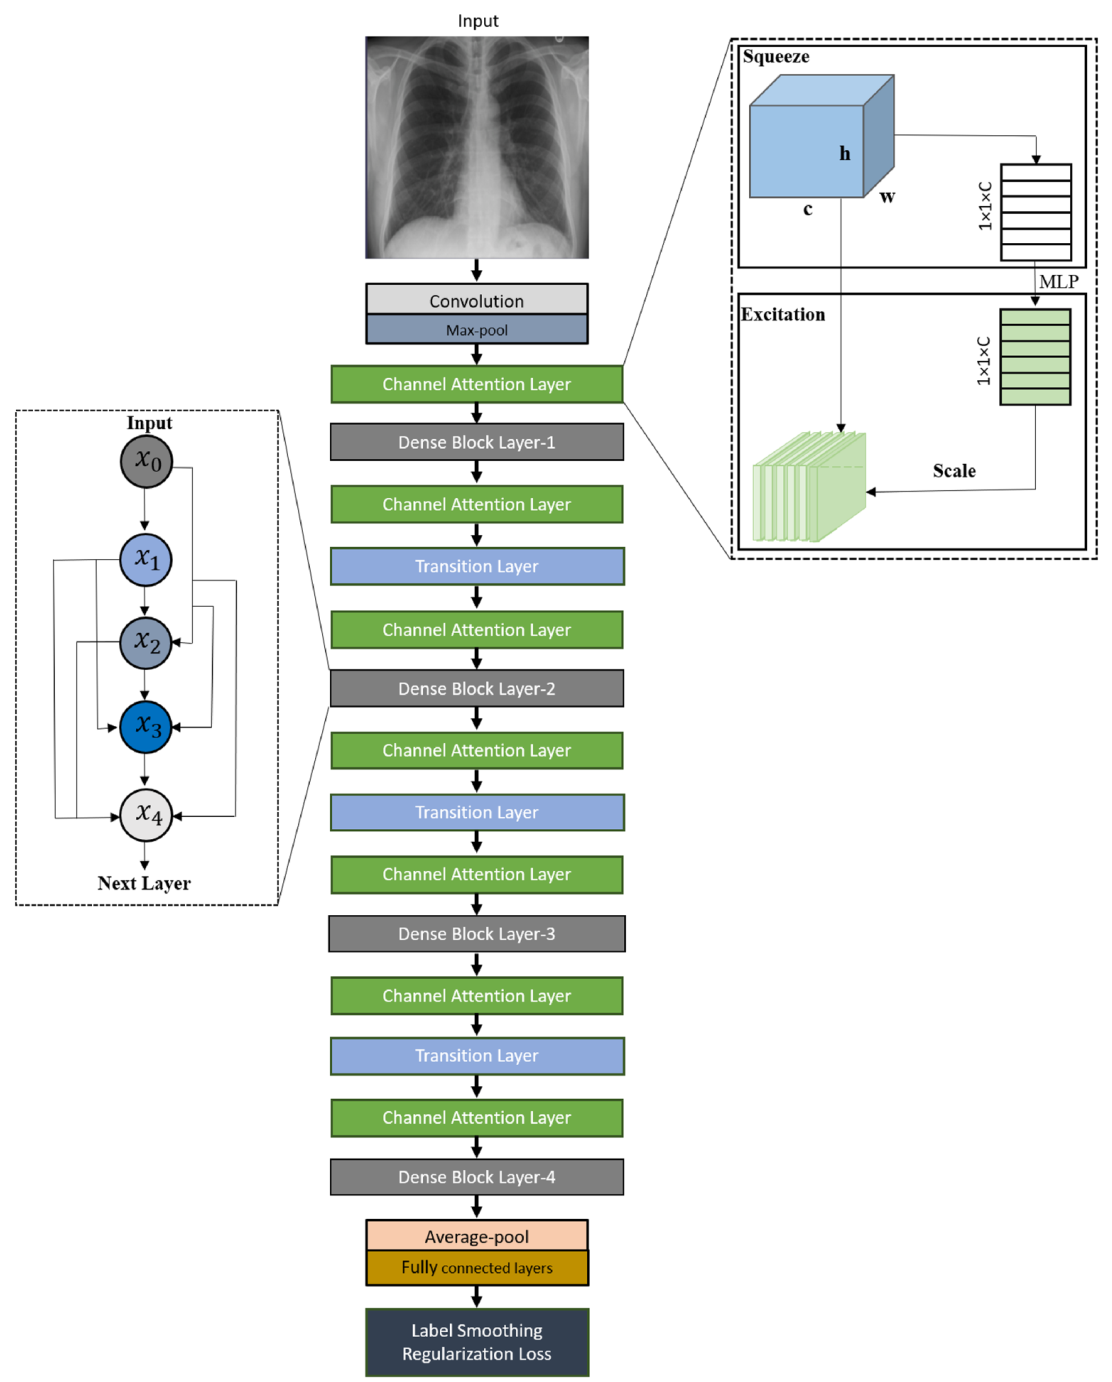
\includegraphics[width=0.5\textwidth]{Densely_attention_mechanism_based_network}
		\bicaption[稠密型注意力机制网络用来检测 COVID-19的感染情况]
			{稠密型注意力机制网络用来检测 COVID-19的感染情况\cite{Ullah2023DenselyAM}}
			{Densely attention mechanism network to detect the COVID-19 infection}
		\label{fig:COVID19}
	\end{figure}
	通过跟正常肺部影像和普通肺炎所造成阴影区域对比,比较明确地指出COVID-19感染区域(图\ref{fig:COVID19_detection}中COVID-19一栏所高亮显示的),展现给临床医生,辅助诊断是否感染新冠肺炎。
	\begin{figure}[ht]
		\centering
		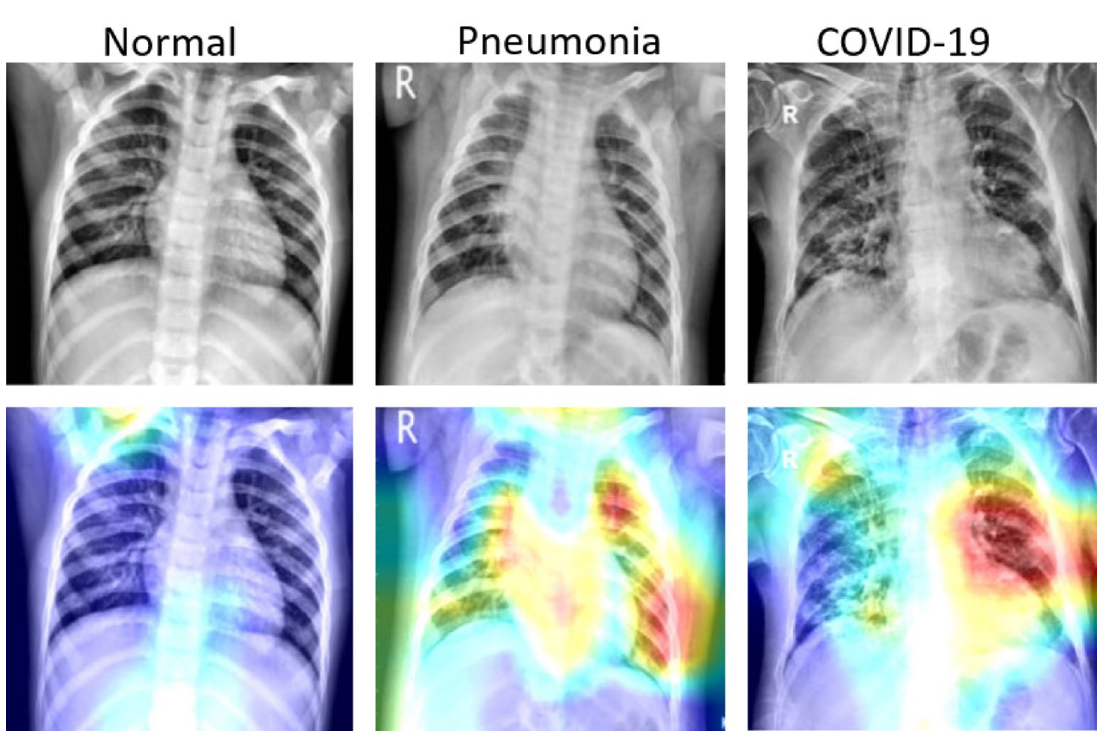
\includegraphics[width=0.4\textwidth]{Detect_COVID19_infection}
		\bicaption[对比正常肺部、普通肺炎和COVID-19新冠肺炎的阴影,突出新冠肺炎感染区域]
			{对比正常肺部、普通肺炎和COVID-19新冠肺炎的阴影,突出新冠肺炎感染区域\cite{Ullah2023DenselyAM}}
			{Highlight the COVID-19 infection area by comparing with normal and pneumonia}
		\label{fig:COVID19_detection}
	\end{figure}
	
	最新的进展是,随着NLP的Transformer模型\cite{Devlin2019BERTPO, NIPS2017Attention}取得成功后,受此启发,NVIDIA的Ali Hatamizadeh联合
	Vanderbilt University的Yucheng Tang等人\cite{unetr}率先将Transformer引入3D medical image segmentation中来,提出了UNETR网络结构
	(见图\ref{fig:UNETR}所示),实现了State-of-the-art (SOTA)医疗图像分割性能新记录。
	\begin{figure}[hbp]
		\centering
		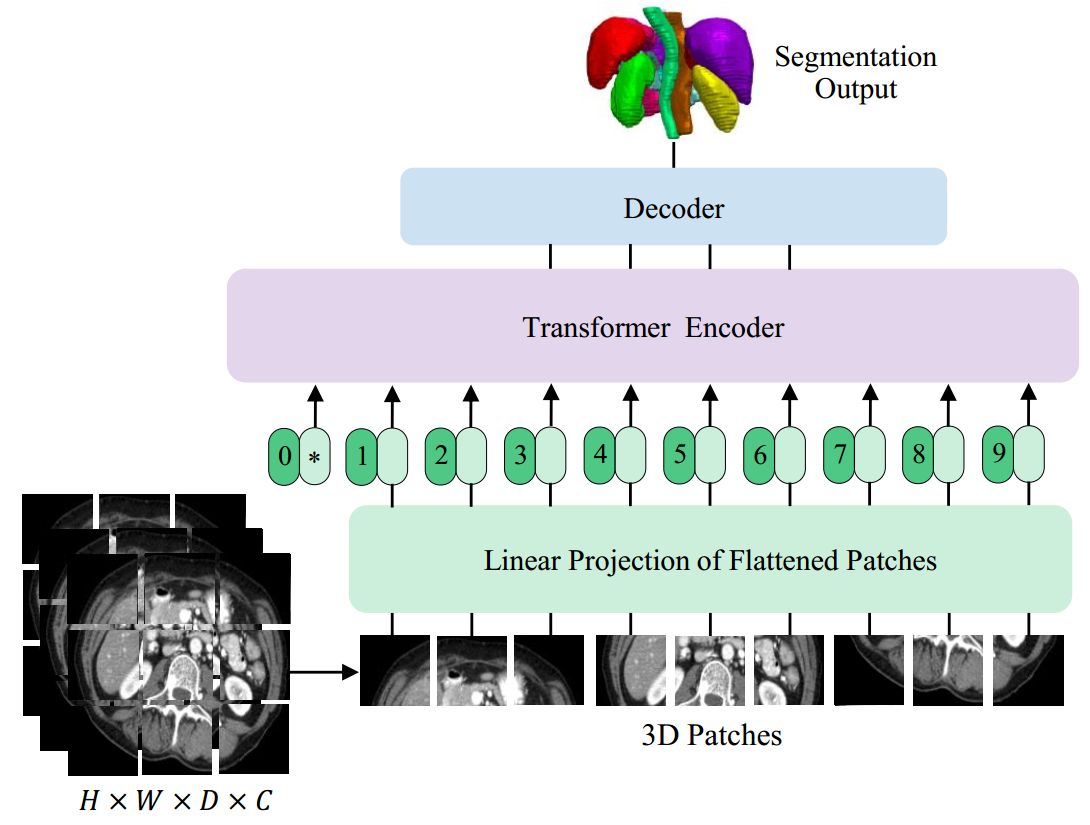
\includegraphics[scale=0.2]{Overview_of_UNETR}
		\bicaption[UNET网络基本结构]
			{UNETR网络基本结构\cite{unetr}}
			{The basic structure of UNETR network}
		\label{fig:UNETR}
	\end{figure}
	
	综上所述,基于深度学习的医疗图像分割技术发展非常活跃,研究进展迅速,进步巨大。
	
	
	
	\subsection{针对肺部支气管气道树的医疗图像分割方法}
	对于肺部CT图像的分割,卷积神经网络CNN早就应用在上面了。最知名的LUng Nodule Analysis 2016大挑战竞赛要求参赛选手分割出Lung CT图像的肺结节,判断肺结节是
	良性的还是恶性的,从而筛选出肺癌疑似患者,进行早期预防和针对性治疗。从LUNA16大挑战竞赛里诞生了两个具有重要影响力的公开数据集LUNA和LIDC-IDRI
	\cite{Charles2011LIDC}。 类似于LUNA	大挑战竞赛,针对肺部支气管气道树的分割也有一个比较著名的EXtraction of Ariways from CT 2009 (EXACT'09)竞赛项目。
	Pechin Lo等人\cite{Lo2012ExtractionOA}在2009年发起了EXACT'09这个竞赛项目,其研究目标就是提供一个公开通用的数据集,鼓励参赛选手开发出创新性算法,从胸部CT扫描
	图像中提取出支气管气道树,评比参赛选手门提交的算法。
	
	自EXACT'09大挑战竞赛的激励后涌现了大量的研究成果, Zhao Tianyi等人\cite{Zhao2019BronchusSA}开发出来一个两阶段2D + 3D的神经网络和一个基于线性规划的气道
	分割跟踪算法。之后2D CNN和2.5D CNN网络相继被提出来,Yun Jihye等人\cite{YUN201913}提出的2.5D卷积网络进行逐个体素分割。在轴向(Axial)、
	矢状(Sagittal)和冠状(Coronal)三个正交方向上取相邻的三个切片,送入2个卷积层的网络,然后将他们合并起来。 这个方法在分割粗支气管时效果还不错,减少了假阳性,检测到
	的气道树的长度也增长了不少。Qier Meng等人\cite{Meng2017TrackingAS}直接采用了3D FCN网络,沿着气道的中心线跟踪气道,并根据每个气道的直径和运行方向设置VOI
	(感兴趣	的立方体体积),3D FCN提取VOI内的气道树,最后将所有的VOI区域内的气道合并为一个完整的气道树。浙江大学医学院第二附属医院的Wu Xiaoming等人
	\cite{Wu2021TACNet}在UNet网络结构的基础上设计了一个Tiny Atrous卷积网络,称为TACNet\cite{Wu2021TACNet}结构(见图\ref{fig:TACNet}),并在EXACT'09数据集
	上对平均Tree Length Detected取得了SOTA性能。
	\begin{figure}[!htp]
		\centering
		\begin{subfigure}{\textwidth}
			\centering
			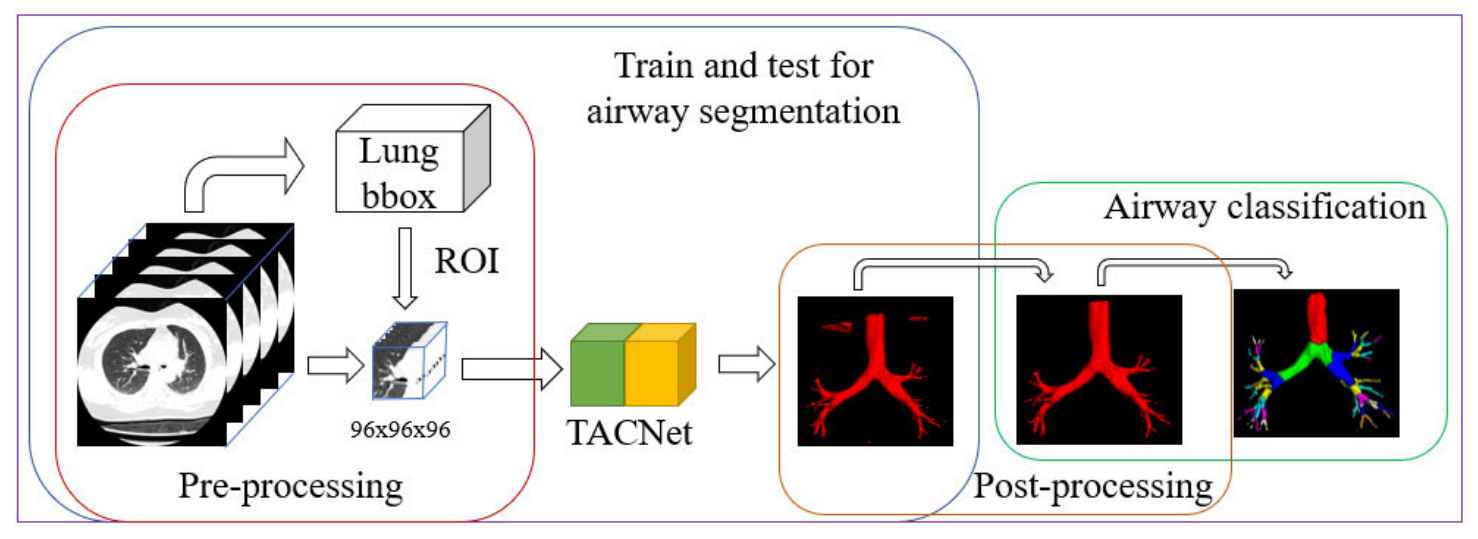
\includegraphics[width=0.5\textwidth]{TACNet_Flowchart}
			\caption{TACNet气道树分割流程}
		\end{subfigure}
		
		\vspace{5mm}
		
		\begin{subfigure}{\textwidth}
			\centering
			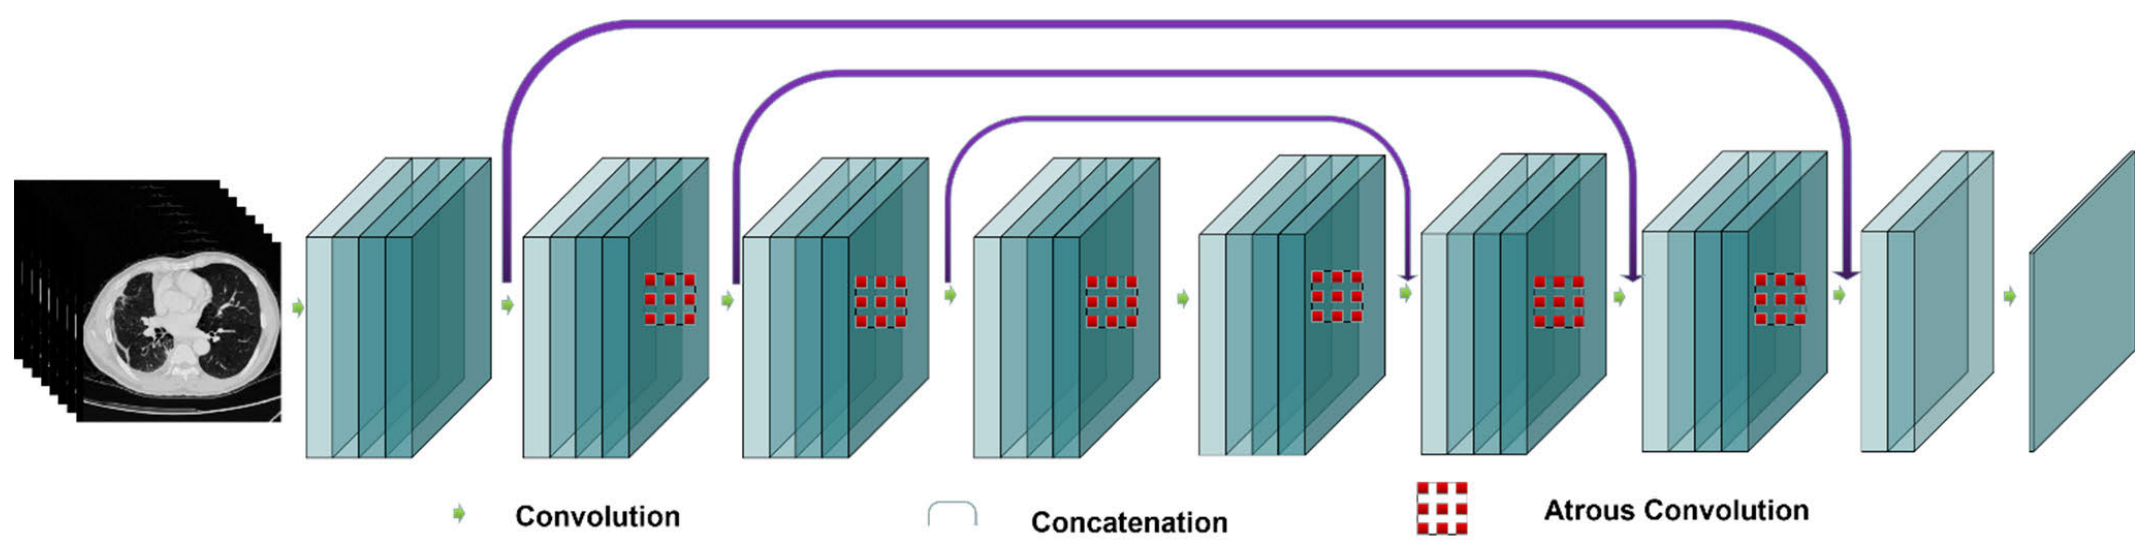
\includegraphics[width=0.7\textwidth]{TACNet_architecture}
			\caption{TACNet网络结构}
		\end{subfigure}
		\bicaption[TACNet气道树分割网络]
			{TACNet气道树分割网络\cite{Wu2021TACNet}}
			{Tiny Atrous Convolution network to segment the airway tree}
		\label{fig:TACNet}
	\end{figure}
	
	以上一些研究成果是基于基础的CNN卷积网络实现了对支气管气道树的分割,在当时提出来时都具有一些创新性,但对分割的精细程度显得不足。他们一般能分割到叶支气管
	(Lobar bronchus),但对于更纤细的段支气管(Segmental bronchi),甚至伸到肺泡的末端小叶支气管(Lobular bronchi),他们已经显得能力不够,难以分割更细小的支气了。
	
	 随着深度学习图像分割技术的发展,更新的技术,更强大的网络结构被开发出来。Guo Jinquan等人\cite{Guo2021CoarsetofineAS}利用多信息融合网络
	 (图\ref{fig:MifCNN}所示)和基于CNN的区域生长网络(图\ref{fig:VCN})相互结合的方式,由粗到细迭代式逐渐分割出更细小的支气管气道树。
	 \begin{figure}[t]
	 	\centering
	 	
	 	\begin{subfigure}{\textwidth}
	 		\centering
	 		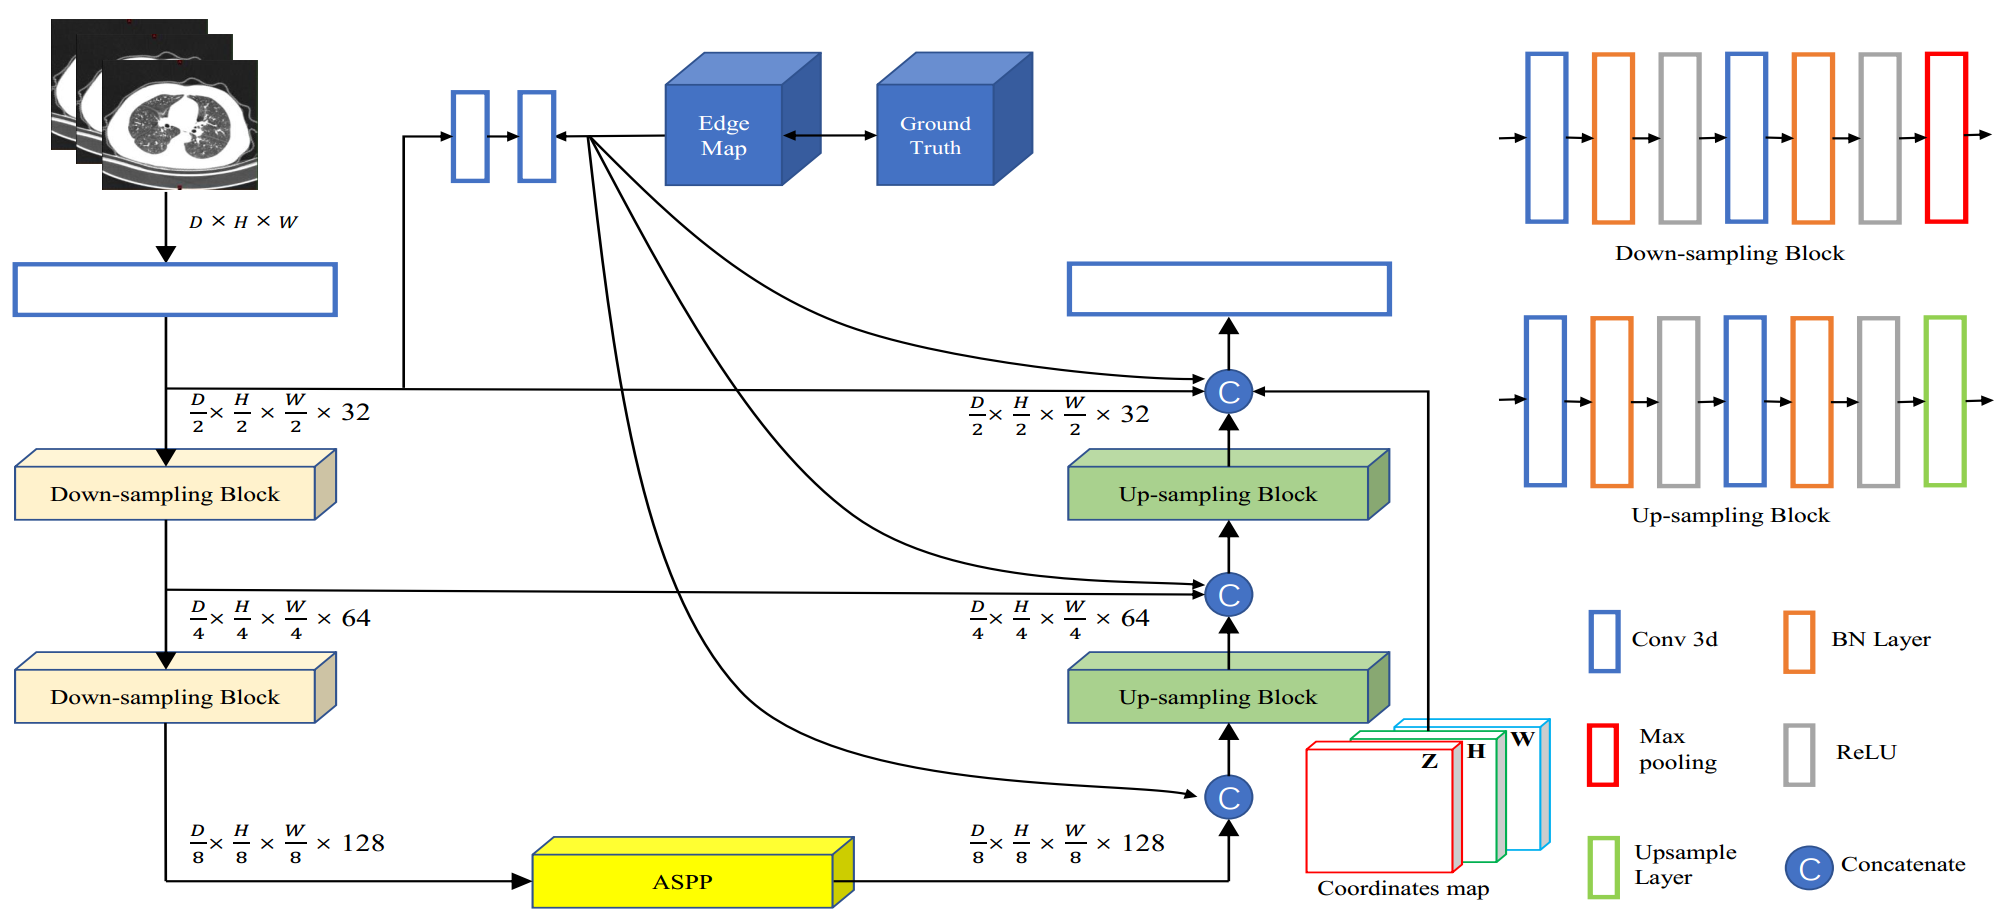
\includegraphics[width=0.7\textwidth]{Mif_CNN}
	 		\caption{多信息融合Mif-CNN网络}
	 		\label{fig:MifCNN}
	 	\end{subfigure}
	 	
	 	\vspace{5mm}
	 	
	 	\begin{subfigure}{\textwidth}
	 		\centering
	 		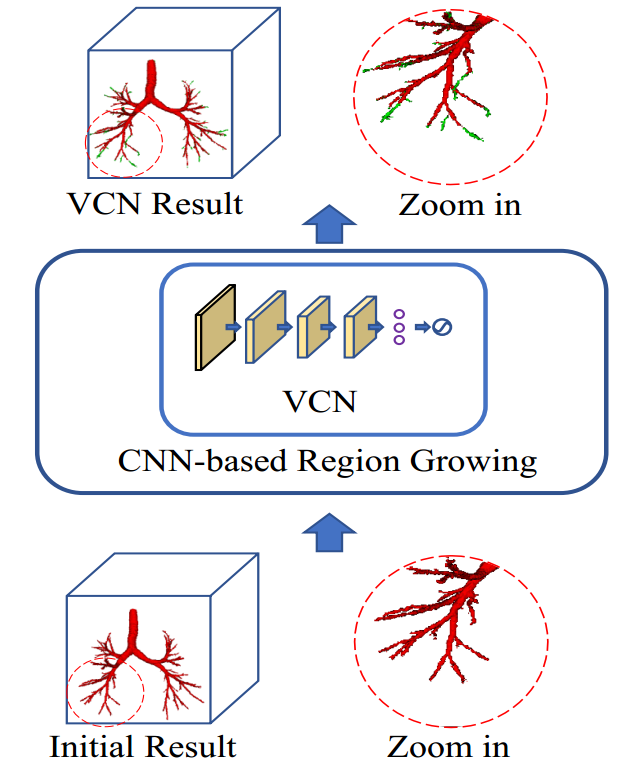
\includegraphics[scale=0.2]{VCN}
	 		\caption{基于CNN的区域生长网络}
	 		\label{fig:VCN}
	 	\end{subfigure}
	 	
	 	\bicaption[多信息融合Mif-CNN网络和基于CNN区域生长网络的组合]
	 		{多信息融合Mif-CNN网络和基于CNN区域生长网络的组合\cite{Guo2021CoarsetofineAS}}
	 		{Corse-to-fine airway segmentation, Mif-CNN and CNN-based region growing combination}
	 \end{figure}
	 
	 肺部支气管气道是一棵树的形状,从CT图像中提取支气管树可视为支气管镜手术导航的细粒度图。上海交通大学医疗机器人研究院的Yu Weihao等人\cite{Yu2022TNN}将图神
	 经网络的概念迁移过来,创新性地提出了一种基于图神经网络的结构,并命名为树网络(Tree Neural Network, TNN)。这种树网络结构巧妙地将支气管分支看成是映射
	 到图空间的节点,提取气道树视为构建节点之间连接的边,也就是支气管分支连接的超边(Hyperedges),见图\ref{fig:TNN}所示。
	 \begin{figure}[htpb]
	 	\centering
	 	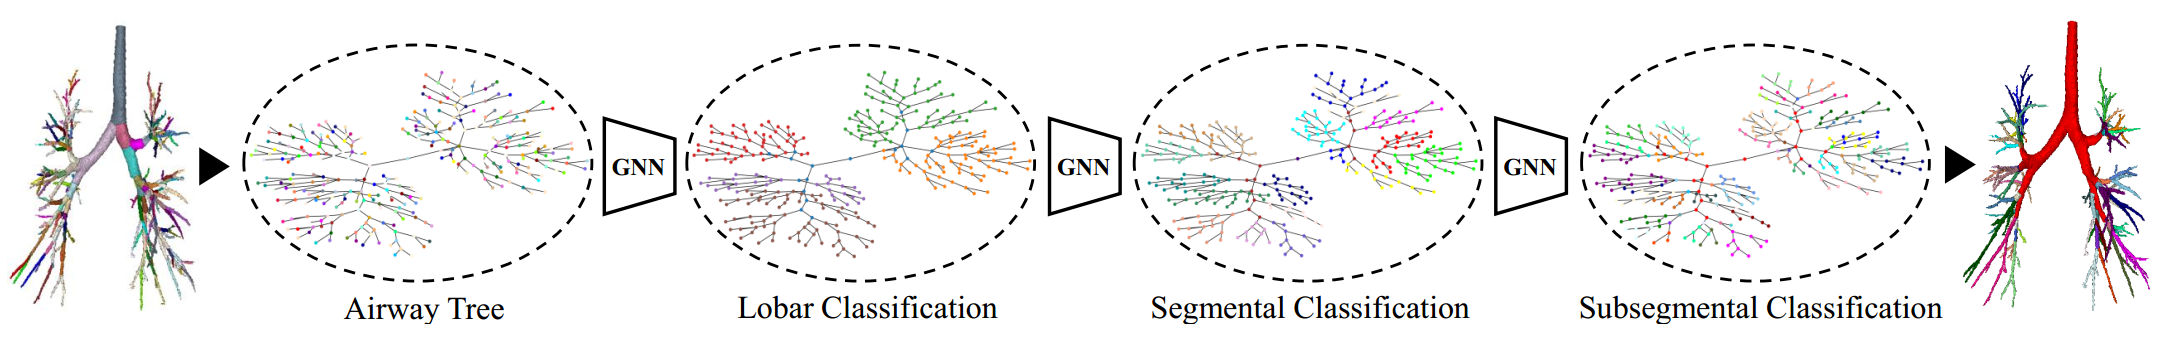
\includegraphics[width=\textwidth]{TNN}
	 	\bicaption[创新性的树网络结构]
	 		{创新性的树网络结构,用GNN来提起支气管气道树\cite{Yu2022TNN}}
	 		{The novel Tree Neural Network, extract the airway tree by virtue of GNN}
		\label{fig:TNN}
	 \end{figure}
	 
	 这种创新性的树网络结构带来了很大的性能提升,尤其对于分割叶支气管、段支气管和小叶支气管的分割分别能达到93.6\%和82.0\%\cite{Yu2022TNN}的精确度。



\section{挑战和困难}

尽管现有的一些研究取得很优秀的成果,肺部支气管气道树的分割性能不断提升,但仍有非常大的挑战需要克服。主要表现在如下方面:
\begin{itemize}
	\item {\heiti 类别严重不平衡}
	
	像肺部支气管、血管、动静脉等管状物体,在CT扫描的切片图像中,前景像素(指支气管管腔、管壁的像素)与背景像素(指除了支气管管腔管壁的像素之外的像素)个数对比
	差别巨大,这就造成严重的类别不平衡。而绝大部分卷积网络都严重依赖标注数据,标注数据缺乏,高质量的标注数据更是稀少,这将导致分割效果大打折扣。肺部树状的支气管、
	肺动脉和肺静脉都是非常纤薄的,在肺部都是发散地分布着。这完全不同于肝脏、肾脏和胰腺这些块状器官\footnote{块状器官指的是肝脏、肾脏和胰腺在CT图像上看起来是一个
	大的区块,非常易于辨认,也容易做区块边缘分割。},标注这些块状器官的前景像素(Pixel)或体素(Voxel)\footnote{注:像素Pixel指在平面图像中一个 高 $\times$ 宽 为
	($H \times W = 1 \times 1$)的平面网格,体素Voxel指的是在CT这样的三维图像上一个 深 $\times$ 高 $\times$ 宽为
	($D \times H \times W = 1 \times 1 \times 1$)的立方体格,其中$D = 1$指的是一个轴向切片的厚度。}与背景像素或体素相差不甚巨大,但对于肺部支气管,标注的
	像素或体素个数与背景像素或体素个数相比则差距悬殊。在单张切片$H \times W = 512 \times 512$这样的高扫描分辨率下,叶支气管Lobar bronchus、段支气管
	Segmental bronchi分别可能只有4个,3个到2个像素,而到肺泡的小叶支气管Lobular bronchi则只有1个像素甚至不到1个像素。这种毛细的管状物不仅加剧了精细标注的难度,
	也导致标注的前景像素与背景像素对比,强烈不平衡。
	
	若卷积网络学习一张$H \times W = 512 \times 512$像素的灰度图像,而标记数据只有两、三个像素。即使将卷积核尺寸(Kernel size)调整到最小,移动步长(Stride)调整
	到最小,最后得到的分割结果其假阳性率(False Positive Rate)也是非常高,精度也是非常差。尽管有加权交叉熵损失Weighted cross-entrophy loss
	\cite{Yuri2019WeightedCrossEntrophy}函数和数据增强Data Augmentation技术,仍难以保证有效地学习到图像的特征信息。
	
	\item {\heiti 全局尺度和局部尺度的上下文信息难以同时兼顾}
	
	肺部支气管是在三维空间上分布的,其众多的分支分散在肺部各处。我们的分割当然不仅仅要学习到气道(Trachea)、左右主支气管(Left/Right main bronchus)、上/中/下肺
	叶支气管(Superior/Middle/Inferior Lobar bronchus)的特征信息,还要学习从上/中/下肺叶支气管扩展出来的段支气管(Segmental bronchi),甚至是延伸至肺泡
	的小叶支气管(Lobular bronchi)的特征信息。细小的支气管这种局部尺度的上下文其实不需要多大的感受野,但对于粗大一些的气道、左右主支气管,我们又需要更大一些的感受野
	来推测整体的气道树形状,也即全局尺度的上下文。面对这种矛盾,应该使用多少个池化层?如果简单地堆积更多的池化层,那么增加的参数可能会因为训练数据不足而导致过拟合。
	如果为了避免这种参数爆炸而牺牲卷积网络的宽度(即特征通道的数量)来换取深度(卷积层的层数),那么模型的学习和拟合能力可能不够\cite{Qin2021TubuleSen}。
	所以,全局尺度的上下文信心与局部尺度的上下文信息是否能够兼顾到呢? 这是另一个困难与挑战之处。
\end{itemize}


\section{本文的研究内容和创新点}

本文针对肺部CT扫描三维图像,建立基于深度学习的三维卷积网络3D-UNet模型\cite{ronneberger2015u}来分割提取人体肺部支气管树状的气道结构。我们使用来自MICCAI2022的
Airway Tree Modeling(ATM) Challenge 2022(以下简写为ATM22\cite{Zhang2022CFDA, Qin2019AirwayNet, Yu2022Bronchi, Zhang2021Airway})的数据集,先将
NiFTI格式的CT扫描三维图像裁剪切成长方体,只保留肺部区域。我们以3D-UNet作为基准模型,做一个基准实验,观察3D-UNet基准模型对支气管气道树的分割效果。研究3D-UNet分割
模型的不足之处,我们提出三点改进方案,也就是本文的创新之处。

\begin{enumerate}

\item {\kaishu 引入一种新的损失函数Focal Loss, 重塑常用的交叉熵损失来解决类别严重不平衡问题}

由于肺部支气管标记数据的稀疏性,造成前景标记像素与背景像素对比严重的类别不平衡。常规的交叉熵Cross-Entrophy Loss损失函数在训练过程中遇到极端的前景和背景类别不平衡时,
分类器对于大量的无分类数据,其权重分配会越来越向这种无分类数据倾斜,而真正拥有分类的数据其获得的权重分配几乎被淹没了,所以导致分类精度下降严重。
新的损失函数Focal Loss则是重塑交叉熵损失函数,使权重分配向有分类的数据倾斜,从而提高分割的精度。

\item {\kaishu 引入注意力蒸馏机制,增加额外的梯度,聚焦于辨识更细小纤薄的支气管}

自NLP研究中提出注意力机制\cite{NIPS2017Attention}后,我们认识到注意力图是在指导网络聚焦看图像的一些重要的地方,这些重要的地方是区分或辨识物体的显著特征。这种有价值
的注意力图可以从教师网络逐层传递到学生网络,从知识蒸馏的角度说,就是知识是可传递的。教师网络学习到知识可以传递到学生网络。我们就是在注意力机制的启发下,将注意力蒸馏机制
引入到我们的3D-UNet网络,在上采样路径上给相邻的两个反卷积层增加一个额外的梯度,使网络聚焦于辨识更细小纤薄的支气管,如段支气管和小叶支气管。

\item {\kaishu 为改善池化层对支气管空间位置信息的捕捉,设计一个再校准模块,用于强化与任务相关的特征,即关键的空间位置信息。}

在下采样路径上池化层收缩,在上采样路径上池化层膨胀,支气管空间位置信息在不同的分辨率下没有被区别对待,池化层没有对支气管空间位置信息有效地捕捉。而这些关键的空间位置信息
对于支气管气道树的精细分割至关重要,因此为了强化于任务相关的特征,为了很好地捕捉支气管的空间位置信息,特地设计一个再校准模块。

\end{enumerate}


\section{论文组织结构}

论文的各个章节安排如下:

{\kaishu 第\ref{chap:introduction}章:\nameref{chap:introduction}}

介绍本论文的研究背景和意义,追踪关于肺部支气管气道树分割这个课题的研究现状和发展趋势。提出本论文的研究内容和有哪些创新点。

{\kaishu 第\ref{chap:baseline_model}章:\nameref{chap:baseline_model}}

阐述3D-UNet基准模型的原理,设计实验对支气管气道树进行分割,研究与展示实验结果,分析不足之处。

{\kaishu 第\ref{chap:attention_distillation}章:\nameref{chap:attention_distillation}}

阐述注意力蒸馏的原理,取下采样路径上四个卷积层的输出结果,进行注意力蒸馏操作,然后对比研究其对分割效果的改进作用。

{\kaishu 第\ref{chap:feature_relearning}章:\nameref{chap:feature_relearning}}

阐述通道级特征再学习的基本原理和计算方法,实现特征再学习模块。将特征再学习模块加到3D-UNet + AD网络进行训练,研究训练的结果,分析评估其对支气管气道树分割的改进效果。
通过一个综合实验展示综合分割效果和指标参数,在验证集和测试集上分割出精确完整的三维气道树结构。

{\kaishu 第\ref{chap:summary_and_outlook}章:\nameref{chap:summary_and_outlook}}

对本文所作的工作进行总结,并对肺部支气管气道树分割这个课题的未来研究方向进行展望。

需要指出的是,本文会穿插着进行对比实验,没有专门的章节来讲解消融研究Ablation Study,消融研究将体现在对比实验中。

\section{本章小结}

本章先介绍了支气管气道树分割课题的研究背景和意义,阐述与课题相关的研究现状和发展状况。 然后就本课题分析指出其挑战性和欲解决的问题,提出论文的创新点。最后展示论文的组织结构和章节安排。


